\section{Features Of Nessi2}
NeSSi2 is designed to extend conventional network simulation tool features by supporting
detailed examination and testing opportunities of security-related network algorithms,
detection units and frameworks. The main focus of NeSSi2 is to provide a
realistic packet-level simulation environment as a testbed for the development of new
detection units as well as existing ones.NeSSi2 has been designed as a modular application with the focus on extensibility. In particular, NeSSi2 provides out-of-the-box support for various protocols of the TCP/IP stack.
\subsection{Traffic Generation}
Network traffic in the form of IP packets, complete with header and body, can be generated by different means. Implementing the TCP/IP protocol stack, NeSSi2 features an application layer module which is based on standard Java socket implementations.

NeSSi2 incorporates several application level protocols (HTTP, SMTP, etc.) and supports
static and dynamic routing protocols which can be selected by the user. At the
moment, static and dynamic protocols are implemented. A static routing protocol centrally computes the shortest paths as the network is loaded and each time the topology changes. The subsequent directing tables are thusly stacked onto the
individual system hubs. Then again, IS-IS(Intermediate- System-to- Intermediate-System) has been
actualized as a connection state convention, which depends on a decentralized calculation amid which
switches trade data about their connection states and assemble topology data locally.
\subsection{Protocol Stack and Socket-based API}
The routers as well as the end devices in the simulation contain a Network Layer; end devices also exclusively have a Transport and an Application Layer. At the Network Layer, IPv4 is realized with the key features global addressing, routing and fragmentation support. Moreover, TCP/IP model implementation allows containing several protocols in each layer; hence, Nessi2 also provide IPv6 support in NeSSi2. For the fault management, TTL (Time to live) and header checksums supported and the ICMP protocol has been implemented for failure notification.

Transport Layer is comprised of UDP and TCP. TCP in NeSSi2 offers a reliable and in-order delivery of data. Sockets represent the interface to the Application Layer, i.e., applications can set up several stream sockets as well as the corresponding server sockets. In this mold, outsider Java libraries can undoubtedly be incorporated in the recreation by substituting Java attachments with NeSSi2 attachments. All applications that are keep running in NeSSi2 take after a typical interface that edited compositions from their particular conduct however permits an institutionalized method for executing them. Right now, the HTTP, SMTP and IRC conventions are incorporated in NeSSi.
\subsection{Security Features}
The simulation setup in NeSSi2 is not only comprised of network creation and attachment
of traffic profiles, but additionally security related settings can be configured.
When a security framework composed of several detection units is to be tested, profiles
can also be used in NeSSi2 to simulate attacker behavior and attack patterns. NeSSi2 provides out-of-the box support for various attack scenarios such as bot networks initiating DDoS attacks. Here, infected end device nodes, “zombies”, are controlled by the bot net commander via the Internet Relay Chat application. The commander is capable of initiating different kinds of DDoS attacks like the SYN Flooding or UDP Storm. To this end, the attacker connects to an IRC communication server and sends attack commands to a chat channel all the bots are listening to. Therefore, the bots execute the coveted assault.
\section{Nessi2 Advantages}
\textbf{1) Scalability} - The user can use JAVA language to write application, and use Maven to define and adds the dependencies of the application. Therefore, Nessi2 can add functionality or application needed.

\textbf{2) Fidelity} - Nessi2 creates a network topology based on network characteristics, it also can automatically generate a network topology depended on the download file, it has high fidelity. (It can download the AS topology file from CAIDA website, then import into Nessi2, automatically generated network topology).

\textbf{3) Extensibility} - Nessi2 can work with third-party software, such as Wireshark.
\section{Components Of Nessi2}
\subsection{Graphical User Interface}

GUI of NeSSi2 has two use cases: On the one hand, results of running or terminated simulations can be visualized in here. On the other hand,
it is the component that allows the creation and modification of network topologies and scenarios.
A project consists of a root folder, some predefined sub folders and some files created by the user. The root folder is named after the project, whereas the sub folders are named after the element types they contain. NeSSi2 project files include the following types: networks, applications, profiles, scenarios, simulations, recorder configurations and the optional templates.
\begin{figure}[h]
	\centering
	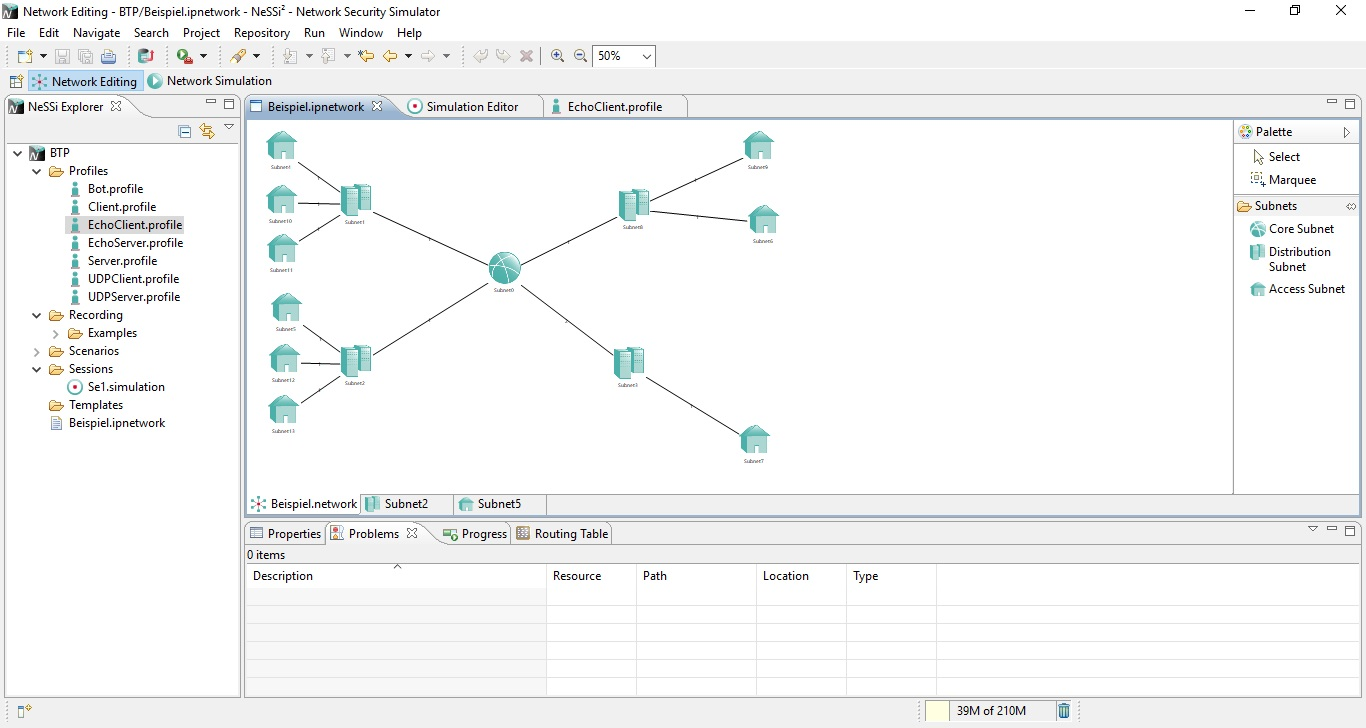
\includegraphics[width=\linewidth]{Nessi2GUI.JPG}
	\caption{GUI Of Nessi2}
	\label{fig:netwok}
\end{figure}

\newpage
\subsection{Simulation Backend}
The genuine reenactment is performed on a machine with equipment committed exclusively to this reason, the recreation backend.Once a reproduction is submitted for execution, the reproduction backend parses the coveted reproduction parameters (which occasion composes to log, what number of rushes to execute and so on.), makes a relating reproduction condition, sets up the database association and calendars the reproduction to keep running when the essential handling assets are accessible.NeSSi2 is built upon the JIAC framework, JIAC is a service-centric java-based middleware architecture based on the agent paradigm. Within NeSSi, agents are used for modeling and implementing the network entities such as routers, clients, and servers. The fundamental JIAC operator system gives a rich and adaptable reason
for actualizing and testing of different security arrangements and calculations in NeSSi2. Besides, expanding upon a specialist system permits joining the fractional information of the operators living in the system in a helpful approach for recognizing and in the end killing IP-based dangers.
\begin{figure}[h]
	\centering
		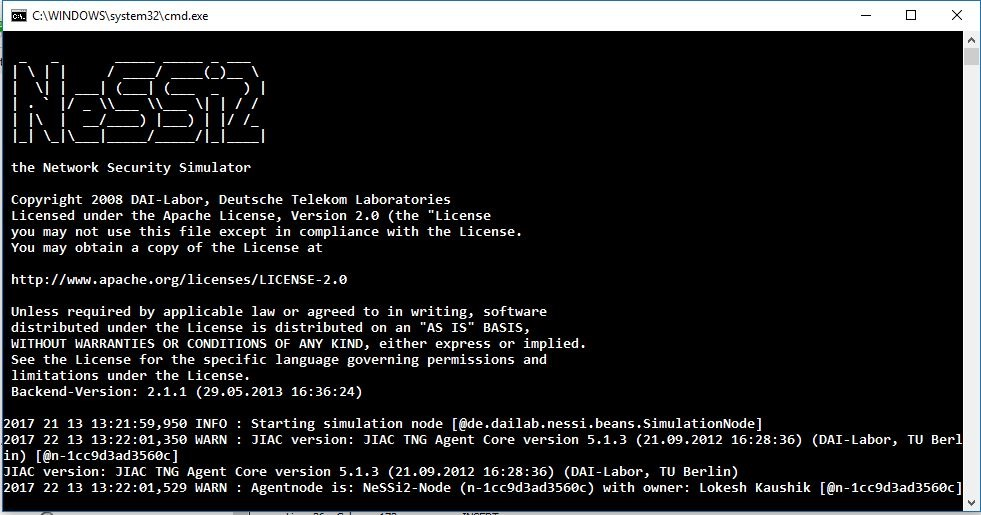
\includegraphics[width=\linewidth]{Backend.JPG}
	\caption{Nessi2 Backend}
	\label{fig:backend}
\end{figure}
\newpage
\subsection{Database}
The exact propagation of a reenactment empowers clients to utilize diverse discovery techniques or different arrangements of location units for a similar activity informational index. This permits the examination of execution and identification proficiency of various security system setups.For these purposes, we use a distributed database in which the traffic generated during a simulation is stored. For each simulation, the agents log the traffic and detection data and send it to the database that occurs in a simulated scenario between a start and end time. The data types to be logged are specified by the user in the simulation parameters.The network model is saved in an XML file.
\newline
Due to the modular design of the database component, the actual implementation of the
database is up to the user. This can be comfortably managed via the graphical user interface, where the location of the database, database user name, password and the database driver can be specified. NeSSi2 has been tested extensively with a MySQL database server, but depending on the user’s preferences, this can easily be substituted by another module.

\section{How we created DDOS simulation}
\subsection{Create Nessi2 Project}
As a first step a NeSSi2 project has to be created using the NeSSi2 project creation
wizard. This wizard can be accessed in two ways in the NeSSi2 GUI. One way is by
the following menu sequence: File-> New-> IP Network(Project).

\begin{figure}[h]
	\centering
	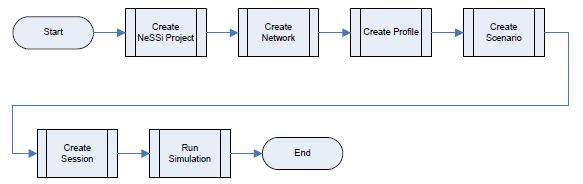
\includegraphics[width=\linewidth]{procedureJPG.JPG}
	\caption{}
	\label{fig:procedure}
\end{figure}
\subsection{create Network}
The nodes and edges of each network are grouped in subnets. Hence, the first step of creating a network is defining some subnets for the network. The available subnet types are listed in the palette located on the right side of the Network Editor Via drag and drop we can add the subnets to the network.
The next step after adding subnets to the network is to add content to the subnets. In
order to do so, double click on a subnet. This will cause for a new tab to be opened
in the Network Editor. Same as with the subnets, the palette will display a list of the
available nodes and edges. By dragging and dropping nodes, they will be added to the
network. For connecting nodes, we will have to select one of the links found in the
Connections part of the palette and than clicking on the nodes that we want to connect.
We also have to connect the subnets to each other. In this case, we  have to select an network element (usually the routers) and enter its context menu. Select Connect to Subnet, then select the subnet we  want to connect to. This will cause for the network device to appear in both subnets.
\begin{figure}
	\centering
	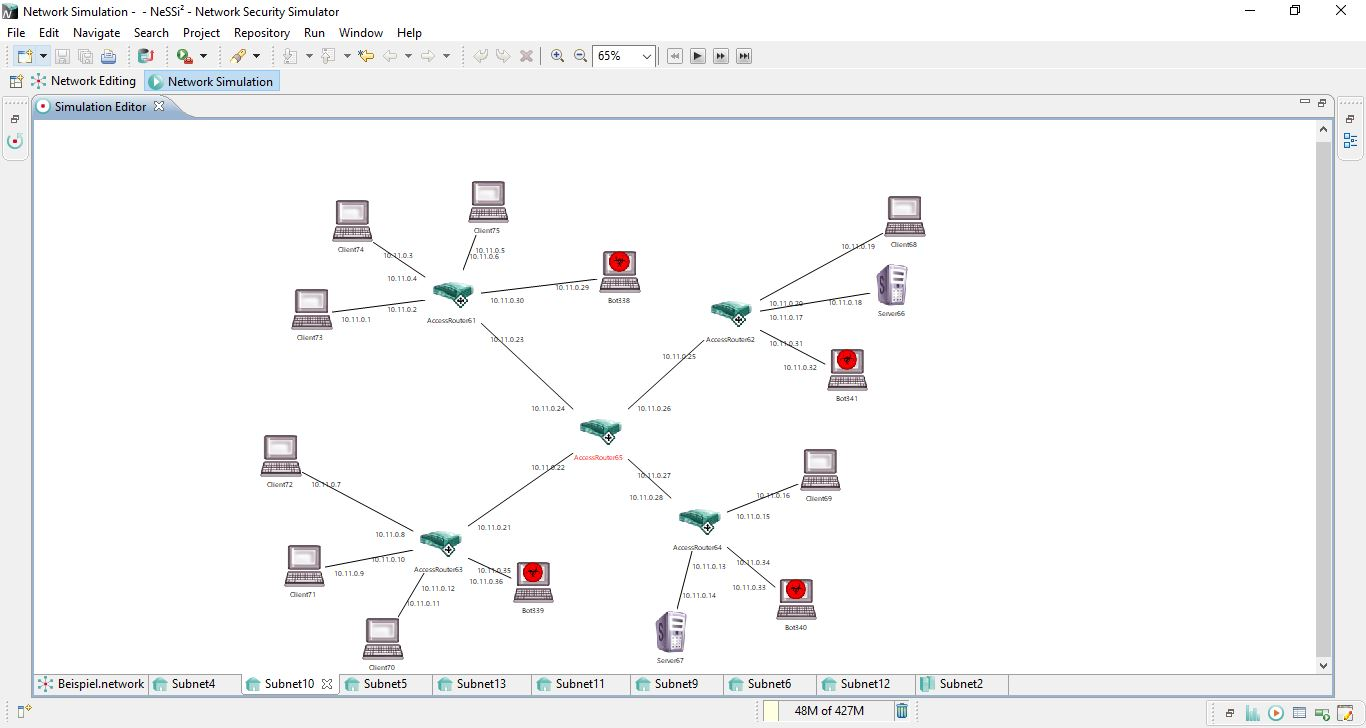
\includegraphics[width=\linewidth]{subnet.JPG}
	\caption{Network design of subnet}
	\label{fig:subnet}
\end{figure}

\newpage
\subsection{Create Profile}
A profile is basically a container for a set of applications.Explorer and selecting New->Profile.This will open a dialog where a name has to be entered for the profile. By pressing "Finish", the dialog will close and a file with the .profile extension will be created in the Profiles folder of the project. Now, applications may be added to the profile.By pressing the Add... button in the newly created profile, we can add applications to the profile.
\subsection{Create Scenario}
A scenario is the mapping of profiles onto the nodes of a specific network.A scenario defines which profiles are deployed on each node of the network topology.
Multiple profiles may be deployed on the same node simultaneously. Analogous to the
profiles, the scenarios are stores in the Scenarios directory of each project with .scenario file extension and XML-based content.
\subsection{Create Simulation}
As the core element of simulation execution, simulations are the components that can be
launched from within the user interface and evaluated in the backend. Simulation files
have .simulation file extension and XML-based content and are located in Sessions
folder of a project.The duration of a simulation execution is determined by two parameters, namely replications and ticks. Replications specify how many times a scenario is to be executed, whereas ticks are the time units by which runs are measured.
\subsection{Recorder Configurations}
Recorder configurations specify the event types that are to be recorded during the simulation execution in NeSSi2 Backend onto the database. The default configurations can
be found in Recordings/Examples folder of each NeSSi2 project.
\newpage
\section{Results and simulation}
\begin{figure}[h]
	\centering
		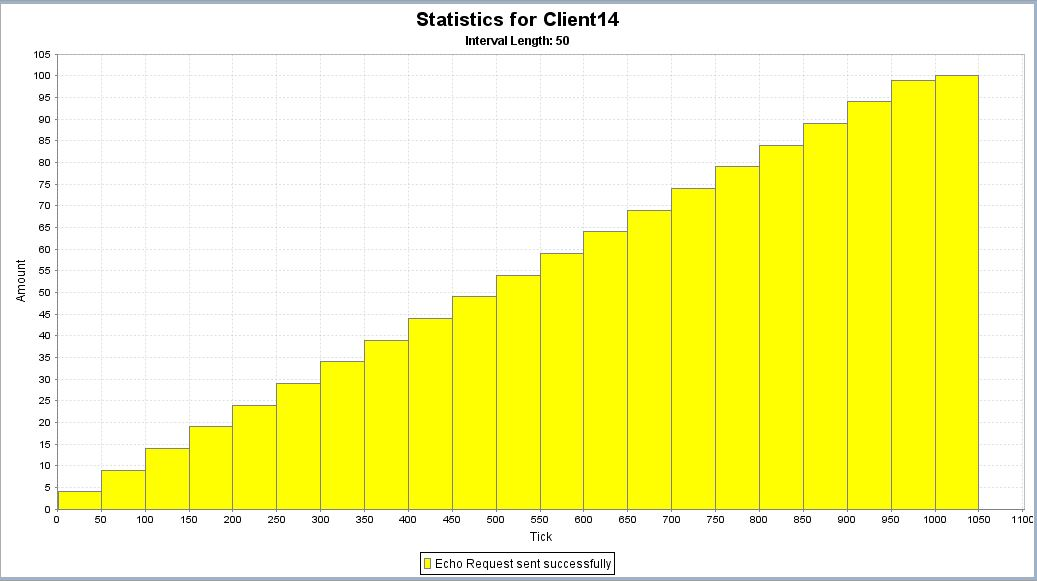
\includegraphics[width=\linewidth]{Client14.JPG}
	\caption{}
	\label{fig:client10}
\end{figure}
\begin{figure}[h]
	\centering
		\includegraphics[width=\linewidth]{Client74.JPG}
	\caption{}
	\label{fig:client13}
\end{figure}
\begin{figure}[h]
	\centering
		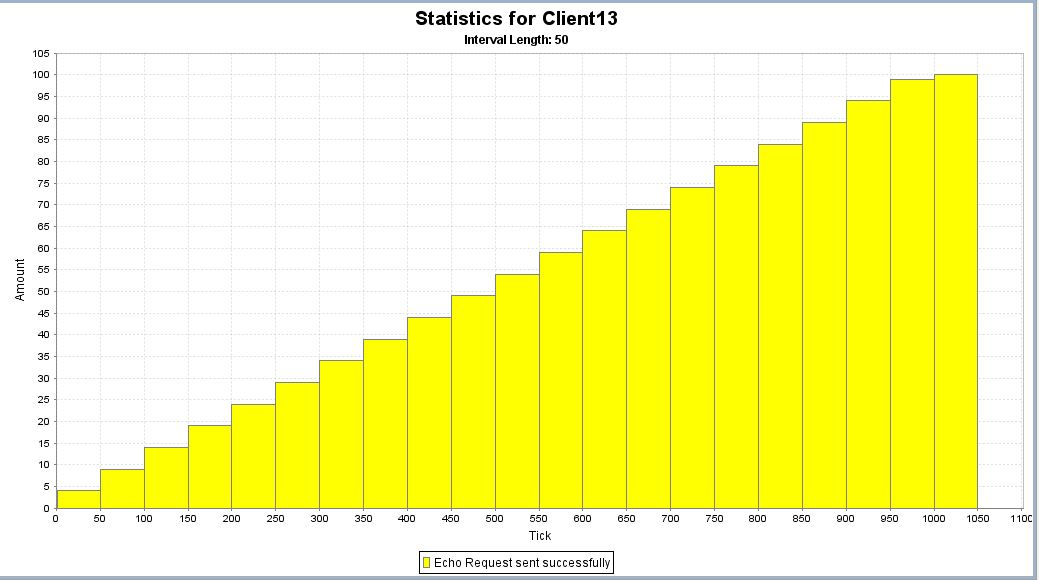
\includegraphics[width=\linewidth]{client.JPG}
	\caption{}
	\label{fig:client54}
\end{figure}










